\section{Atomistic modelling and simulation of dislocation avalanches }
The magnitude of time scale in molecular dynamics (MD) simulation can hardly go beyond nanoseconds, which is magnitudes away from real time experiments. To over come this disadvantage we use an alternative approach of exploring the structure of the energy landscape and identifying the transition pathway and barrier. This information is incorporated in TST calculations. Many atomistic algorithms are developed like activation-relaxation technique (ART) and autonomous basin climbing (ABC) method to incorporate the energy barriers and pinning points .$^{\cite{Fan2020}}$

Slip avalanches also known as discrete stress relaxations and are strain-rate sensitive.The modelling of constant strain-rate simulation is done using transition state expression is given equ. (\ref{transition_equ}) $^{\cite{Fan2020}}$


\begin{equation}\label{transition_equ}
\dot{\varepsilon}=\dot{\gamma}_{0} \exp \left(-E_{b} / k_{\mathrm{B}} T\right)
\end{equation}


For atomistic modelling, The following step are to be performed:


\begin{itemize}
  \item Energy minimization i.e the local energy of the system is minimum. For each iteration the energy minimization is performed to the system to equilibrium. 
  
  \item Atomistic algorithms like ABC or ART must be applied to the system to generate local energy barriers and pinning points which are essential for dislocation avalanches.
  
  \item External load is applied and for small strain rate, the energy state is configured and saved
  
  \item The stored atomic configuration are used to calculate the single-atom displacement and strains.
  
\item For each iteration, energy minimization with respect to the external load need to be achieved for the iteration to terminate. This process is continued till a maximum  strain is achieved.
\end{itemize}

\begin{wrapfigure}{R}{0.3\textwidth}
\centering
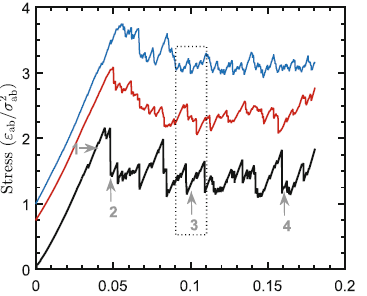
\includegraphics[width=0.35\textwidth]{section_3_1.png}
\caption{\label{fig:Simulation graph}stress-strain graph.$^{\cite{Fan2020}}$}
\end{wrapfigure}


After reaching maximum strain, the subsequent
plastic flow is essentially dominated by this shear localized region, involving sliding
and thickening. 

The figure (\ref{fig:Simulation graph}) show the response of strains for different strain-rates.For all the strain-rates, the material shows elasticity till yield point represented by point 1.Then at point 2 there is sudden drop in stress due to impending of dislocation.A significant sharpening of stress is observed in plasticity.This variation of stress with strain-rate is called over-shooting. This signifies that the dislocation avalanches result in strain bursts.$^{\cite{Fan2020}}$

The dislocation statistics and there implications on stress-strains are discussed in the next section.